\documentclass[11pt]{article}

\usepackage[margin=1in]{geometry}
\usepackage{setspace}
\usepackage{graphicx}
\usepackage{booktabs}
\usepackage[colorlinks=true, linkcolor=blue, urlcolor=blue]{hyperref}
\usepackage{float}
\usepackage{xcolor}
\usepackage{amsmath}

\graphicspath{{output/graphs/}}

\title{Heterogeneous Results: College vs.\ Non-college\\
       \large Split-sample DiD --- March 17, 2026}
\author{Leyao Wang}
\date{}

\begin{document}
\maketitle
\thispagestyle{empty}

\noindent\textit{College} = BA or above (educ $>$ 110). \textit{Non-college} = high school or some college (educ $\leq$ 110). All regressions estimated on the CPS-ASEC 2018--2025 sample of labor-force participants aged 22--65 with at least a high school diploma. AI exposure is the Eloundou et al.\ (2024) GPT-4 beta score. Year 2022 is the omitted baseline throughout.

\bigskip

%==================================================
\section*{Contents}
%==================================================

\subsection*{Combined plots (college vs.\ non-college on one axis)}
\begin{enumerate}
  \item \hyperref[fig:unemp_naive_colComb]{Unemployment: Naive --- college vs.\ non-college}
  \item \hyperref[fig:unemp_sexFE_colComb]{Unemployment: Sex FE --- college vs.\ non-college}
  \item \hyperref[fig:unemp_sexeducFE_colComb]{Unemployment: Sex + Education FE --- college vs.\ non-college}
  \item \hyperref[fig:lw_naive_colComb]{Log Wage: Naive --- college vs.\ non-college}
  \item \hyperref[fig:lw_sexFE_colComb]{Log Wage: Sex FE --- college vs.\ non-college}
  \item \hyperref[fig:lw_sexeducFE_colComb]{Log Wage: Sex + Education FE --- college vs.\ non-college}
\end{enumerate}

\subsection*{Unemployment regression tables}
\begin{enumerate}\setcounter{enumi}{6}
  \item \hyperref[tab:unemp_A_col]{Unemployment Table A (double interaction) --- college}
  \item \hyperref[tab:unemp_A_noncol]{Unemployment Table A (double interaction) --- non-college}
  \item \hyperref[tab:unemp_B_col]{Unemployment Table B (experience triple interaction) --- college}
  \item \hyperref[tab:unemp_B_noncol]{Unemployment Table B (experience triple interaction) --- non-college}
\end{enumerate}

\subsection*{Log wage regression tables}
\begin{enumerate}\setcounter{enumi}{10}
  \item \hyperref[tab:lw_A_col]{Log Wage Table A (double interaction) --- college}
  \item \hyperref[tab:lw_A_noncol]{Log Wage Table A (double interaction) --- non-college}
  \item \hyperref[tab:lw_B_col]{Log Wage Table B (experience triple interaction) --- college}
  \item \hyperref[tab:lw_B_noncol]{Log Wage Table B (experience triple interaction) --- non-college}
\end{enumerate}

\subsection*{Unemployment coefficient plots --- separate subsamples}
\begin{enumerate}\setcounter{enumi}{14}
  \item \hyperref[fig:unemp_naive_col]{Unemployment: Naive --- college}
  \item \hyperref[fig:unemp_naive_noncol]{Unemployment: Naive --- non-college}
  \item \hyperref[fig:unemp_sexFE_col]{Unemployment: Sex FE --- college}
  \item \hyperref[fig:unemp_sexFE_noncol]{Unemployment: Sex FE --- non-college}
  \item \hyperref[fig:unemp_sexeducFE_col]{Unemployment: Sex + Education FE --- college}
  \item \hyperref[fig:unemp_sexeducFE_noncol]{Unemployment: Sex + Education FE --- non-college}
\end{enumerate}

\subsection*{Log wage coefficient plots --- separate subsamples}
\begin{enumerate}\setcounter{enumi}{20}
  \item \hyperref[fig:lw_naive_col]{Log Wage: Naive --- college}
  \item \hyperref[fig:lw_naive_noncol]{Log Wage: Naive --- non-college}
  \item \hyperref[fig:lw_sexFE_col]{Log Wage: Sex FE --- college}
  \item \hyperref[fig:lw_sexFE_noncol]{Log Wage: Sex FE --- non-college}
  \item \hyperref[fig:lw_sexeducFE_col]{Log Wage: Sex + Education FE --- college}
  \item \hyperref[fig:lw_sexeducFE_noncol]{Log Wage: Sex + Education FE --- non-college}
\end{enumerate}

\subsection*{DiD unemployment scatter}
\begin{enumerate}\setcounter{enumi}{26}
  \item \hyperref[fig:delta_col]{DiD unemployment $(u_{2024}-u_{2023})-(u_{2023}-u_{2022})$ vs.\ AI exposure --- college}
  \item \hyperref[fig:delta_noncol]{DiD unemployment $(u_{2024}-u_{2023})-(u_{2023}-u_{2022})$ vs.\ AI exposure --- non-college}
\end{enumerate}

\clearpage
\doublespacing

%==================================================
\section{Combined Coefficient Plots: College vs.\ Non-college}
%==================================================

\begin{figure}[H]
\begin{center}
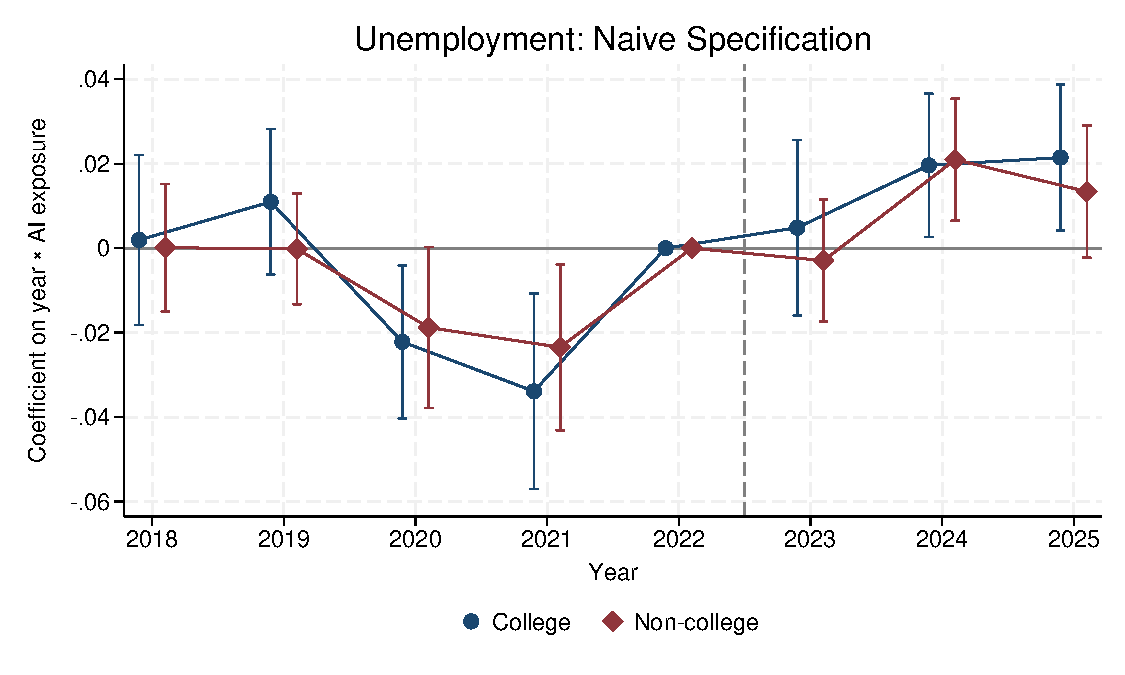
\includegraphics[width=0.88\textwidth]{unemp_naive_plot_colComb.pdf}
\caption{Unemployment: DiD coefficients (year $\times$ AI exposure), naive specification. College-educated workers (BA or above) in navy circles; non-college workers (high school or some college) in maroon diamonds. Year 2022 is the baseline ($\hat\beta_{2022}\equiv 0$).}
\label{fig:unemp_naive_colComb}
\end{center}
\smallskip
\noindent\footnotesize\textit{Notes:} Coefficients from separate-sample OLS regressions of a binary unemployment indicator on (year $\times$ AI exposure), with year 2022 omitted. No additional controls. Error bars are 95\% confidence intervals; standard errors clustered at the occupation level. Horizontal jitter of $\pm0.1$ years applied for readability.
\end{figure}

\begin{figure}[H]
\begin{center}
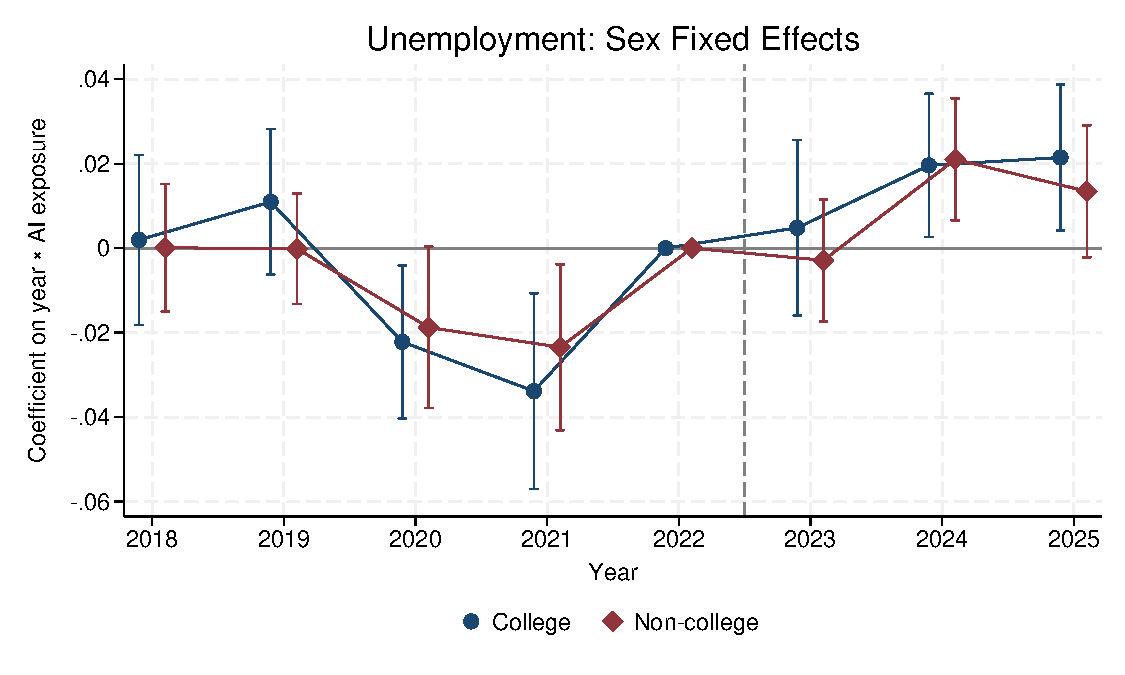
\includegraphics[width=0.88\textwidth]{unemp_sexFE_plot_colComb.pdf}
\caption{Unemployment: DiD coefficients (year $\times$ AI exposure), sex fixed effects. College (navy circles) vs.\ non-college (maroon diamonds). Year 2022 is the baseline.}
\label{fig:unemp_sexFE_colComb}
\end{center}
\smallskip
\noindent\footnotesize\textit{Notes:} Same as Figure~\ref{fig:unemp_naive_colComb} with sex fixed effects absorbed. Standard errors clustered at the occupation level.
\end{figure}

\begin{figure}[H]
\begin{center}
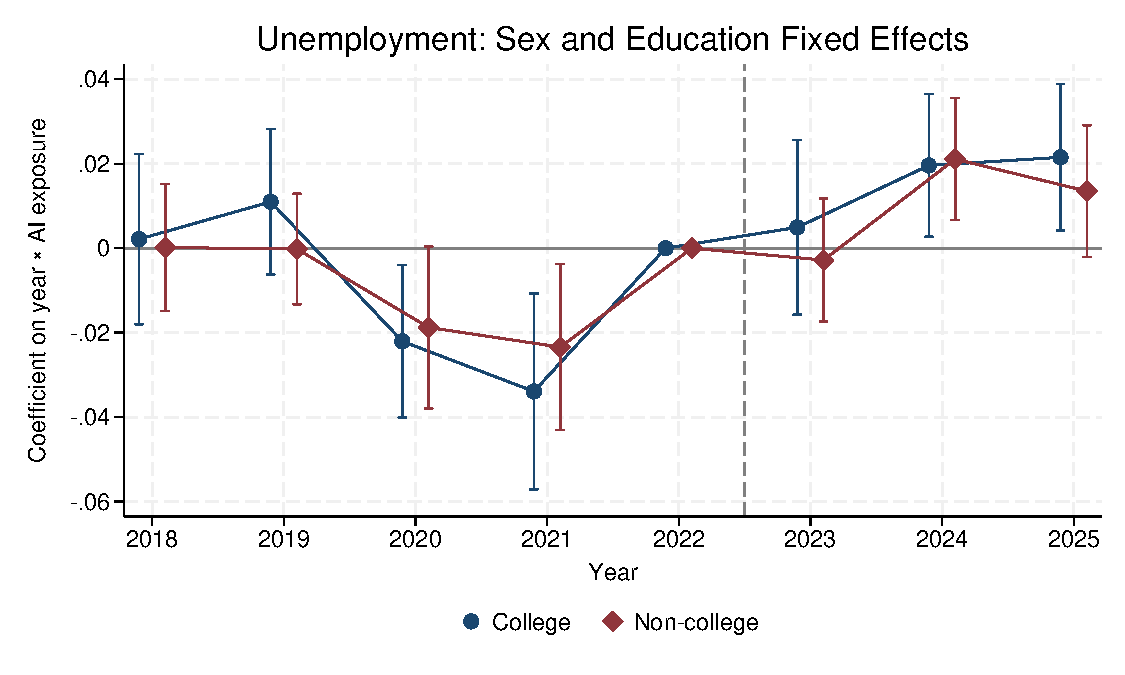
\includegraphics[width=0.88\textwidth]{unemp_sexeducFE_plot_colComb.pdf}
\caption{Unemployment: DiD coefficients (year $\times$ AI exposure), sex and education fixed effects. College (navy circles) vs.\ non-college (maroon diamonds). Year 2022 is the baseline.}
\label{fig:unemp_sexeducFE_colComb}
\end{center}
\smallskip
\noindent\footnotesize\textit{Notes:} Same as Figure~\ref{fig:unemp_naive_colComb} with sex and education fixed effects absorbed. Standard errors clustered at the occupation level.
\end{figure}

\begin{figure}[H]
\begin{center}
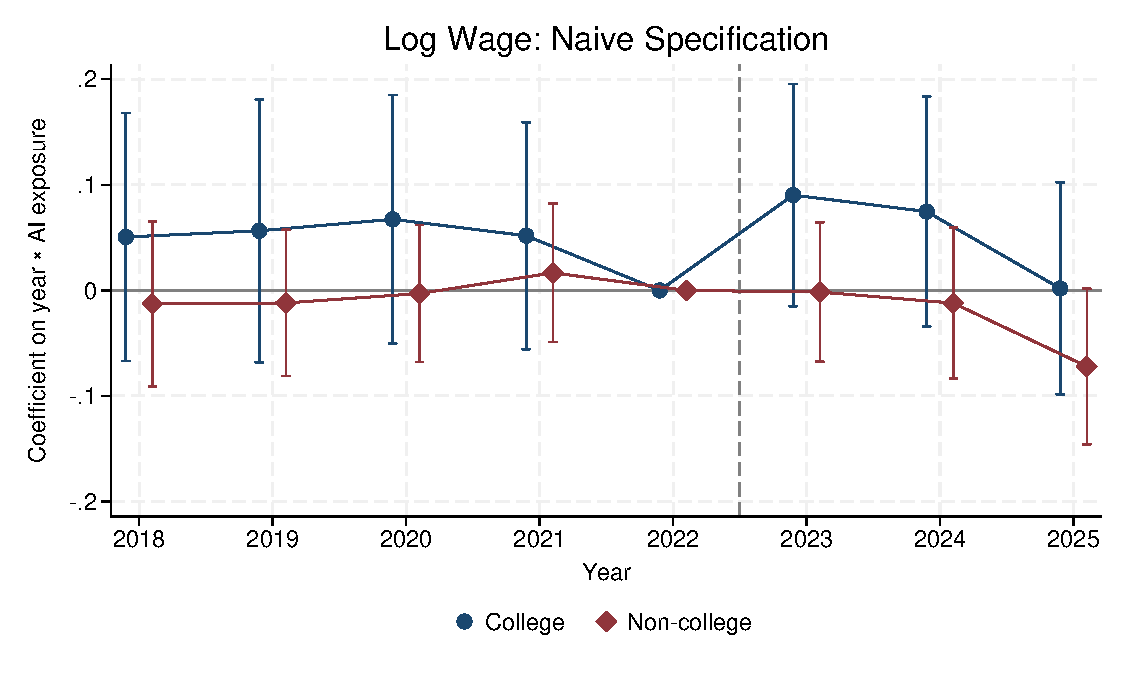
\includegraphics[width=0.88\textwidth]{lw_naive_plot_colComb.pdf}
\caption{Log Wage: DiD coefficients (year $\times$ AI exposure), naive specification. College (navy circles) vs.\ non-college (maroon diamonds). Year 2022 is the baseline ($\hat\beta_{2022}\equiv 0$).}
\label{fig:lw_naive_colComb}
\end{center}
\smallskip
\noindent\footnotesize\textit{Notes:} Coefficients from separate-sample OLS regressions of log annual real wages on (year $\times$ AI exposure), with year 2022 omitted. No additional controls. Observations with zero or missing wage income excluded. Error bars are 95\% confidence intervals; standard errors clustered at the occupation level.
\end{figure}

\begin{figure}[H]
\begin{center}
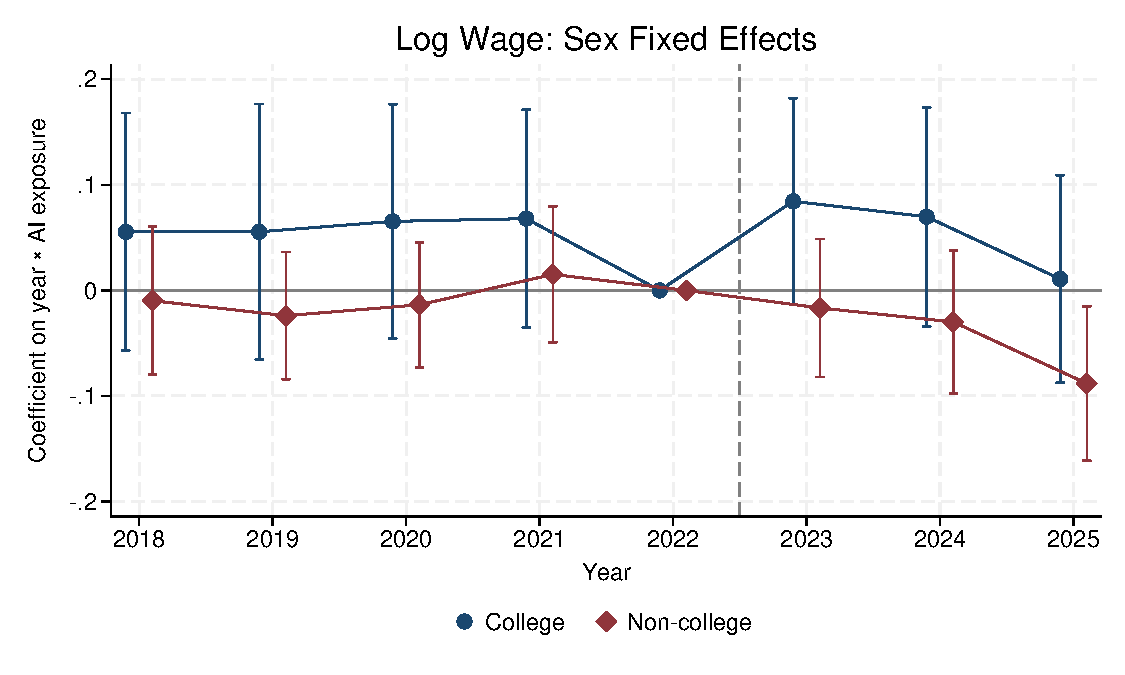
\includegraphics[width=0.88\textwidth]{lw_sexFE_plot_colComb.pdf}
\caption{Log Wage: DiD coefficients (year $\times$ AI exposure), sex fixed effects. College (navy circles) vs.\ non-college (maroon diamonds). Year 2022 is the baseline.}
\label{fig:lw_sexFE_colComb}
\end{center}
\smallskip
\noindent\footnotesize\textit{Notes:} Same as Figure~\ref{fig:lw_naive_colComb} with sex fixed effects absorbed. Standard errors clustered at the occupation level.
\end{figure}

\begin{figure}[H]
\begin{center}
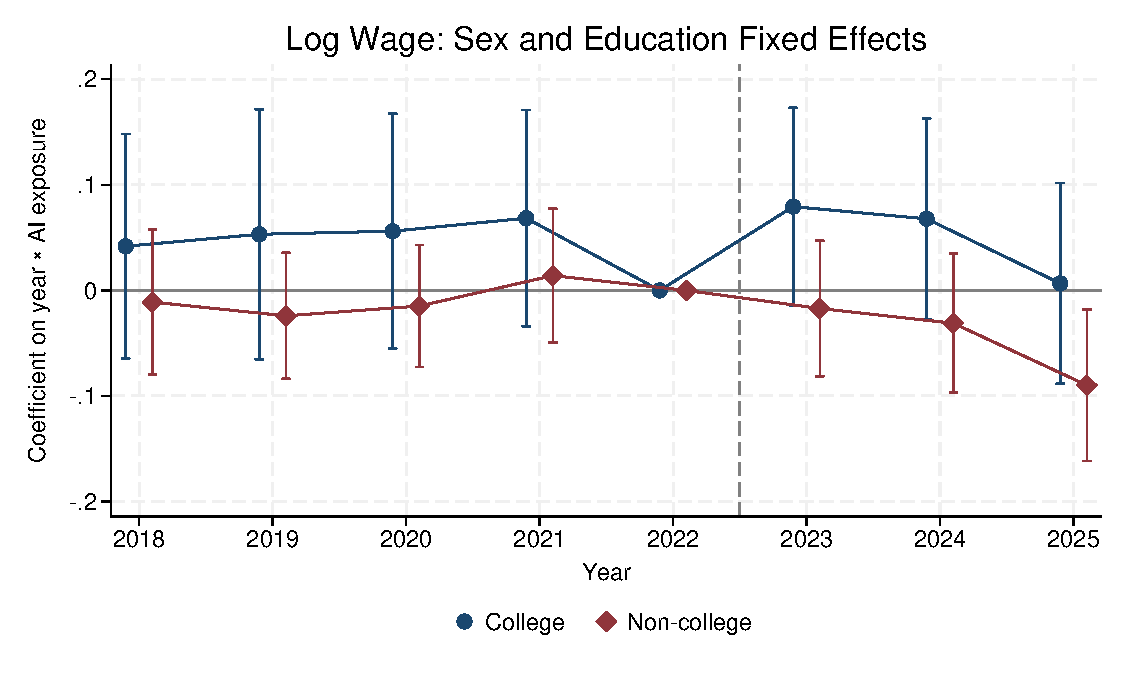
\includegraphics[width=0.88\textwidth]{lw_sexeducFE_plot_colComb.pdf}
\caption{Log Wage: DiD coefficients (year $\times$ AI exposure), sex and education fixed effects. College (navy circles) vs.\ non-college (maroon diamonds). Year 2022 is the baseline.}
\label{fig:lw_sexeducFE_colComb}
\end{center}
\smallskip
\noindent\footnotesize\textit{Notes:} Same as Figure~\ref{fig:lw_naive_colComb} with sex and education fixed effects absorbed. Standard errors clustered at the occupation level.
\end{figure}

\clearpage

%==================================================
\section{Unemployment Regression Tables}
%==================================================

\begin{table}[H]
\begin{center}
\caption{Unemployment Table A --- college subsample. Dependent variable: binary unemployment indicator. Columns (1)--(3): no fixed effects, sex FE, sex + education FE. Year 2022 is the omitted baseline. Standard errors clustered at the occupation level. $^{*}p<0.10$, $^{**}p<0.05$, $^{***}p<0.01$.}
\label{tab:unemp_A_col}
\resizebox{0.9\textwidth}{!}{\def\sym#1{\ifmmode^{#1}\else\(^{#1}\)\fi}
\begin{tabular}{l*{4}{c}}
\toprule
Dependent Variable: & \multicolumn{4}{c}{Unemployment} \\
\cmidrule(lr){2-5}
 & (1) & (2) & (3) & (4) \\
\midrule
2018 $\times$ AI exposure&     0.00194   &     0.00196   &     0.00213   &     0.00209   \\
            &    (0.0102)   &    (0.0102)   &    (0.0102)   &    (0.0104)   \\
2019 $\times$ AI exposure&      0.0110   &      0.0110   &      0.0110   &      0.0106   \\
            &   (0.00877)   &   (0.00876)   &   (0.00875)   &   (0.00875)   \\
2020 $\times$ AI exposure&     -0.0222** &     -0.0222** &     -0.0220** &     -0.0222** \\
            &   (0.00921)   &   (0.00922)   &   (0.00921)   &   (0.00922)   \\
2021 $\times$ AI exposure&     -0.0339***&     -0.0338***&     -0.0339***&     -0.0356***\\
            &    (0.0118)   &    (0.0118)   &    (0.0118)   &    (0.0118)   \\
2023 $\times$ AI exposure&     0.00484   &     0.00482   &     0.00492   &     0.00390   \\
            &    (0.0106)   &    (0.0106)   &    (0.0105)   &    (0.0102)   \\
2024 $\times$ AI exposure&      0.0196** &      0.0196** &      0.0196** &      0.0186** \\
            &   (0.00863)   &   (0.00863)   &   (0.00860)   &   (0.00853)   \\
2025 $\times$ AI exposure&      0.0215** &      0.0215** &      0.0215** &      0.0184** \\
            &   (0.00879)   &   (0.00879)   &   (0.00882)   &   (0.00877)   \\
\midrule
Mean of dependent variable&       0.022   &       0.022   &       0.022   &       0.022   \\
Sex FE      &          No   &         Yes   &         Yes   &         Yes   \\
Education FE&          No   &          No   &         Yes   &         Yes   \\
State $\times$ Year FE&          No   &          No   &          No   &         Yes   \\
SE clustered at&  Occupation   &  Occupation   &  Occupation   &  Occupation   \\
Observations&     221,543   &     221,543   &     221,543   &     221,543   \\
\bottomrule
\end{tabular}
}
\end{center}
\smallskip
\noindent\footnotesize\textit{Notes:} Sample restricted to college-educated workers (BA or above, educ $>$ 110) aged 22--65 in the labor force. Reported coefficients are on the interaction of year dummies with the Eloundou et al.\ (2024) GPT-4 beta exposure score (\texttt{dv\_rating\_beta}).
\end{table}

\begin{table}[H]
\begin{center}
\caption{Unemployment Table A --- non-college subsample. Dependent variable: binary unemployment indicator. Columns (1)--(3): no fixed effects, sex FE, sex + education FE. Year 2022 is the omitted baseline. Standard errors clustered at the occupation level. $^{*}p<0.10$, $^{**}p<0.05$, $^{***}p<0.01$.}
\label{tab:unemp_A_noncol}
\resizebox{0.9\textwidth}{!}{\def\sym#1{\ifmmode^{#1}\else\(^{#1}\)\fi}
\begin{tabular}{l*{4}{c}}
\toprule
Dependent Variable: & \multicolumn{4}{c}{Unemployment} \\
\cmidrule(lr){2-5}
 & (1) & (2) & (3) & (4) \\
\midrule
2018 $\times$ AI exposure&    0.000113   &   0.0000963   &    0.000159   &   0.0000625   \\
            &   (0.00767)   &   (0.00767)   &   (0.00767)   &   (0.00768)   \\
2019 $\times$ AI exposure&   -0.000183   &   -0.000142   &   -0.000203   &   -0.000849   \\
            &   (0.00666)   &   (0.00665)   &   (0.00666)   &   (0.00652)   \\
2020 $\times$ AI exposure&     -0.0188*  &     -0.0188*  &     -0.0188*  &     -0.0184*  \\
            &   (0.00971)   &   (0.00972)   &   (0.00974)   &   (0.00973)   \\
2021 $\times$ AI exposure&     -0.0235** &     -0.0235** &     -0.0234** &     -0.0242** \\
            &   (0.00999)   &   (0.00999)   &    (0.0100)   &   (0.00992)   \\
2023 $\times$ AI exposure&    -0.00294   &    -0.00286   &    -0.00282   &    -0.00346   \\
            &   (0.00737)   &   (0.00734)   &   (0.00739)   &   (0.00732)   \\
2024 $\times$ AI exposure&      0.0210***&      0.0210***&      0.0211***&      0.0206***\\
            &   (0.00735)   &   (0.00734)   &   (0.00735)   &   (0.00732)   \\
2025 $\times$ AI exposure&      0.0134*  &      0.0135*  &      0.0135*  &      0.0135*  \\
            &   (0.00796)   &   (0.00795)   &   (0.00794)   &   (0.00791)   \\
\midrule
Mean of dependent variable&       0.043   &       0.043   &       0.043   &       0.043   \\
Sex FE      &          No   &         Yes   &         Yes   &         Yes   \\
Education FE&          No   &          No   &         Yes   &         Yes   \\
State $\times$ Year FE&          No   &          No   &          No   &         Yes   \\
SE clustered at&  Occupation   &  Occupation   &  Occupation   &  Occupation   \\
Observations&     279,126   &     279,126   &     279,126   &     279,126   \\
\bottomrule
\end{tabular}
}
\end{center}
\smallskip
\noindent\footnotesize\textit{Notes:} Sample restricted to non-college workers (high school or some college, educ $\leq$ 110) aged 22--65 in the labor force. Reported coefficients are on the interaction of year dummies with the Eloundou et al.\ (2024) GPT-4 beta exposure score.
\end{table}

\begin{table}[H]
\begin{center}
\caption{Unemployment Table B --- college subsample. Dependent variable: binary unemployment indicator. Reported coefficients are on the triple interaction year $\times$ potential experience $\times$ AI exposure. Columns (1)--(3): no fixed effects, sex FE, sex + education FE. $F$-test $p$-value tests joint significance of the 2024 and 2025 triple-interaction terms. Standard errors clustered at the occupation level. $^{*}p<0.10$, $^{**}p<0.05$, $^{***}p<0.01$.}
\label{tab:unemp_B_col}
\resizebox{0.9\textwidth}{!}{\def\sym#1{\ifmmode^{#1}\else\(^{#1}\)\fi}
\begin{tabular}{l*{4}{c}}
\toprule
Dependent Variable: & \multicolumn{4}{c}{Unemployment} \\
\cmidrule(lr){2-5}
 & (1) & (2) & (3) & (4) \\
\midrule
2018 $\times$ Experience $\times$ AI exposure&    0.000660   &    0.000657   &    0.000633   &    0.000628   \\
            &  (0.000727)   &  (0.000727)   &  (0.000728)   &  (0.000726)   \\
2019 $\times$ Experience $\times$ AI exposure&    0.000971   &    0.000968   &    0.000974   &     0.00102   \\
            &  (0.000760)   &  (0.000760)   &  (0.000760)   &  (0.000759)   \\
2020 $\times$ Experience $\times$ AI exposure&    0.000314   &    0.000311   &    0.000310   &    0.000345   \\
            &  (0.000879)   &  (0.000880)   &  (0.000878)   &  (0.000885)   \\
2021 $\times$ Experience $\times$ AI exposure&     0.00121   &     0.00121   &     0.00121   &     0.00134   \\
            &  (0.000974)   &  (0.000975)   &  (0.000975)   &  (0.000969)   \\
2023 $\times$ Experience $\times$ AI exposure&    0.000758   &    0.000752   &    0.000761   &    0.000812   \\
            &  (0.000818)   &  (0.000818)   &  (0.000818)   &  (0.000814)   \\
2024 $\times$ Experience $\times$ AI exposure&    0.000571   &    0.000567   &    0.000563   &    0.000648   \\
            &  (0.000925)   &  (0.000926)   &  (0.000922)   &  (0.000919)   \\
2025 $\times$ Experience $\times$ AI exposure&    0.000473   &    0.000469   &    0.000477   &    0.000524   \\
            &  (0.000803)   &  (0.000804)   &  (0.000801)   &  (0.000808)   \\
\midrule
Mean of dependent variable&       0.022   &       0.022   &       0.022   &       0.022   \\
Sex FE      &          No   &         Yes   &         Yes   &         Yes   \\
Education FE&          No   &          No   &         Yes   &         Yes   \\
State $\times$ Year FE&          No   &          No   &          No   &         Yes   \\
SE clustered at&  Occupation   &  Occupation   &  Occupation   &  Occupation   \\
Observations&     221,543   &     221,543   &     221,543   &     221,543   \\
\bottomrule
\end{tabular}
}
\end{center}
\smallskip
\noindent\footnotesize\textit{Notes:} College subsample (educ $>$ 110). Potential experience imputed as $\max(\text{age} - \text{years of schooling} - 6,\, 0)$. A positive (negative) coefficient indicates that higher-experience workers within the college group are more (less) affected by AI exposure relative to lower-experience workers.
\end{table}

\begin{table}[H]
\begin{center}
\caption{Unemployment Table B --- non-college subsample. Dependent variable: binary unemployment indicator. Reported coefficients are on the triple interaction year $\times$ potential experience $\times$ AI exposure. Columns (1)--(3): no fixed effects, sex FE, sex + education FE. Standard errors clustered at the occupation level. $^{*}p<0.10$, $^{**}p<0.05$, $^{***}p<0.01$.}
\label{tab:unemp_B_noncol}
\resizebox{0.9\textwidth}{!}{\def\sym#1{\ifmmode^{#1}\else\(^{#1}\)\fi}
\begin{tabular}{l*{4}{c}}
\toprule
Dependent Variable: & \multicolumn{4}{c}{Unemployment} \\
\cmidrule(lr){2-5}
 & (1) & (2) & (3) & (4) \\
\midrule
2018 $\times$ Experience $\times$ AI exposure&    0.000346   &    0.000344   &    0.000359   &    0.000367   \\
            &  (0.000494)   &  (0.000494)   &  (0.000497)   &  (0.000497)   \\
2019 $\times$ Experience $\times$ AI exposure&    0.000570   &    0.000568   &    0.000583   &    0.000578   \\
            &  (0.000442)   &  (0.000442)   &  (0.000446)   &  (0.000449)   \\
2020 $\times$ Experience $\times$ AI exposure&    0.000602   &    0.000602   &    0.000650*  &    0.000609   \\
            &  (0.000383)   &  (0.000383)   &  (0.000385)   &  (0.000383)   \\
2021 $\times$ Experience $\times$ AI exposure&    0.000793*  &    0.000793*  &    0.000796*  &    0.000812*  \\
            &  (0.000463)   &  (0.000463)   &  (0.000466)   &  (0.000460)   \\
2023 $\times$ Experience $\times$ AI exposure&    0.000241   &    0.000242   &    0.000218   &    0.000182   \\
            &  (0.000443)   &  (0.000444)   &  (0.000444)   &  (0.000444)   \\
2024 $\times$ Experience $\times$ AI exposure&   -0.000164   &   -0.000163   &   -0.000179   &   -0.000196   \\
            &  (0.000523)   &  (0.000523)   &  (0.000525)   &  (0.000524)   \\
2025 $\times$ Experience $\times$ AI exposure&    0.000229   &    0.000231   &    0.000208   &    0.000226   \\
            &  (0.000498)   &  (0.000499)   &  (0.000503)   &  (0.000495)   \\
\midrule
Mean of dependent variable&       0.043   &       0.043   &       0.043   &       0.043   \\
Sex FE      &          No   &         Yes   &         Yes   &         Yes   \\
Education FE&          No   &          No   &         Yes   &         Yes   \\
State $\times$ Year FE&          No   &          No   &          No   &         Yes   \\
SE clustered at&  Occupation   &  Occupation   &  Occupation   &  Occupation   \\
Observations&     279,126   &     279,126   &     279,126   &     279,126   \\
\bottomrule
\end{tabular}
}
\end{center}
\smallskip
\noindent\footnotesize\textit{Notes:} Non-college subsample (educ $\leq$ 110). Potential experience imputed as $\max(\text{age} - \text{years of schooling} - 6,\, 0)$. Note that years-of-schooling imputation is missing for some college codes, so experience is missing for a portion of the non-college sample and those observations are dropped from the triple-interaction regressions.
\end{table}

\clearpage

%==================================================
\section{Log Wage Regression Tables}
%==================================================

\begin{table}[H]
\begin{center}
\caption{Log Wage Table A --- college subsample. Dependent variable: log annual real wages (1982 dollars). Columns (1)--(3): no fixed effects, sex FE, sex + education FE. Year 2022 is the omitted baseline. Standard errors clustered at the occupation level. $^{*}p<0.10$, $^{**}p<0.05$, $^{***}p<0.01$.}
\label{tab:lw_A_col}
\resizebox{0.9\textwidth}{!}{\def\sym#1{\ifmmode^{#1}\else\(^{#1}\)\fi}
\begin{tabular}{l*{4}{c}}
\toprule
Dependent Variable: & \multicolumn{4}{c}{Log Wage} \\
\cmidrule(lr){2-5}
 & (1) & (2) & (3) & (4) \\
\midrule
2018 $\times$ AI exposure&      0.0505   &      0.0554   &      0.0418   &      0.0417   \\
            &    (0.0598)   &    (0.0572)   &    (0.0541)   &    (0.0540)   \\
2019 $\times$ AI exposure&      0.0565   &      0.0555   &      0.0531   &      0.0488   \\
            &    (0.0633)   &    (0.0616)   &    (0.0603)   &    (0.0592)   \\
2020 $\times$ AI exposure&      0.0674   &      0.0654   &      0.0561   &      0.0497   \\
            &    (0.0599)   &    (0.0565)   &    (0.0566)   &    (0.0580)   \\
2021 $\times$ AI exposure&      0.0518   &      0.0680   &      0.0684   &      0.0621   \\
            &    (0.0547)   &    (0.0525)   &    (0.0521)   &    (0.0538)   \\
2023 $\times$ AI exposure&      0.0903*  &      0.0844*  &      0.0793*  &      0.0713   \\
            &    (0.0536)   &    (0.0497)   &    (0.0476)   &    (0.0482)   \\
2024 $\times$ AI exposure&      0.0747   &      0.0697   &      0.0678   &      0.0655   \\
            &    (0.0554)   &    (0.0528)   &    (0.0483)   &    (0.0483)   \\
2025 $\times$ AI exposure&     0.00189   &      0.0108   &     0.00671   &    0.000559   \\
            &    (0.0511)   &    (0.0500)   &    (0.0484)   &    (0.0497)   \\
\midrule
Mean of dependent variable&      10.054   &      10.054   &      10.054   &      10.054   \\
Sex FE      &          No   &         Yes   &         Yes   &         Yes   \\
Education FE&          No   &          No   &         Yes   &         Yes   \\
State $\times$ Year FE&          No   &          No   &          No   &         Yes   \\
SE clustered at&  Occupation   &  Occupation   &  Occupation   &  Occupation   \\
Observations&     208,928   &     208,928   &     208,928   &     208,928   \\
\bottomrule
\end{tabular}
}
\end{center}
\smallskip
\noindent\footnotesize\textit{Notes:} College subsample (educ $>$ 110). Observations with zero or missing \texttt{incwage} excluded. Real wages deflated using annual CPI-U from FRED. Reported coefficients are on the interaction of year dummies with the Eloundou et al.\ (2024) GPT-4 beta exposure score.
\end{table}

\begin{table}[H]
\begin{center}
\caption{Log Wage Table A --- non-college subsample. Dependent variable: log annual real wages (1982 dollars). Columns (1)--(3): no fixed effects, sex FE, sex + education FE. Year 2022 is the omitted baseline. Standard errors clustered at the occupation level. $^{*}p<0.10$, $^{**}p<0.05$, $^{***}p<0.01$.}
\label{tab:lw_A_noncol}
\resizebox{0.9\textwidth}{!}{\def\sym#1{\ifmmode^{#1}\else\(^{#1}\)\fi}
\begin{tabular}{l*{4}{c}}
\toprule
Dependent Variable: & \multicolumn{4}{c}{Log Wage} \\
\cmidrule(lr){2-5}
 & (1) & (2) & (3) & (4) \\
\midrule
2018 $\times$ AI exposure&     -0.0127   &    -0.00971   &     -0.0111   &     -0.0102   \\
            &    (0.0397)   &    (0.0356)   &    (0.0350)   &    (0.0350)   \\
2019 $\times$ AI exposure&     -0.0118   &     -0.0239   &     -0.0241   &     -0.0234   \\
            &    (0.0352)   &    (0.0306)   &    (0.0304)   &    (0.0301)   \\
2020 $\times$ AI exposure&    -0.00295   &     -0.0136   &     -0.0148   &     -0.0141   \\
            &    (0.0330)   &    (0.0301)   &    (0.0295)   &    (0.0297)   \\
2021 $\times$ AI exposure&      0.0166   &      0.0152   &      0.0140   &      0.0122   \\
            &    (0.0334)   &    (0.0327)   &    (0.0323)   &    (0.0317)   \\
2023 $\times$ AI exposure&    -0.00155   &     -0.0166   &     -0.0171   &     -0.0187   \\
            &    (0.0336)   &    (0.0333)   &    (0.0327)   &    (0.0328)   \\
2024 $\times$ AI exposure&     -0.0120   &     -0.0299   &     -0.0311   &     -0.0309   \\
            &    (0.0364)   &    (0.0343)   &    (0.0335)   &    (0.0333)   \\
2025 $\times$ AI exposure&     -0.0720*  &     -0.0882** &     -0.0898** &     -0.0933***\\
            &    (0.0375)   &    (0.0372)   &    (0.0365)   &    (0.0361)   \\
\midrule
Mean of dependent variable&       9.471   &       9.471   &       9.471   &       9.471   \\
Sex FE      &          No   &         Yes   &         Yes   &         Yes   \\
Education FE&          No   &          No   &         Yes   &         Yes   \\
State $\times$ Year FE&          No   &          No   &          No   &         Yes   \\
SE clustered at&  Occupation   &  Occupation   &  Occupation   &  Occupation   \\
Observations&     255,372   &     255,372   &     255,372   &     255,372   \\
\bottomrule
\end{tabular}
}
\end{center}
\smallskip
\noindent\footnotesize\textit{Notes:} Non-college subsample (educ $\leq$ 110). Observations with zero or missing \texttt{incwage} excluded. Real wages deflated using annual CPI-U from FRED. Reported coefficients are on the interaction of year dummies with the Eloundou et al.\ (2024) GPT-4 beta exposure score.
\end{table}

\begin{table}[H]
\begin{center}
\caption{Log Wage Table B --- college subsample. Dependent variable: log annual real wages. Reported coefficients are on the triple interaction year $\times$ potential experience $\times$ AI exposure. Columns (1)--(3): no fixed effects, sex FE, sex + education FE. Standard errors clustered at the occupation level. $^{*}p<0.10$, $^{**}p<0.05$, $^{***}p<0.01$.}
\label{tab:lw_B_col}
\resizebox{0.9\textwidth}{!}{\def\sym#1{\ifmmode^{#1}\else\(^{#1}\)\fi}
\begin{tabular}{l*{4}{c}}
\toprule
Dependent Variable: & \multicolumn{4}{c}{Log Wage} \\
\cmidrule(lr){2-5}
 & (1) & (2) & (3) & (4) \\
\midrule
2018 $\times$ Experience $\times$ AI exposure&     0.00346   &     0.00258   &     0.00300   &     0.00285   \\
            &   (0.00538)   &   (0.00530)   &   (0.00516)   &   (0.00511)   \\
2019 $\times$ Experience $\times$ AI exposure&     0.00591   &     0.00489   &     0.00390   &     0.00434   \\
            &   (0.00477)   &   (0.00476)   &   (0.00467)   &   (0.00463)   \\
2020 $\times$ Experience $\times$ AI exposure&     0.00106   &    0.000288   &   -0.000260   &    0.000163   \\
            &   (0.00419)   &   (0.00424)   &   (0.00422)   &   (0.00420)   \\
2021 $\times$ Experience $\times$ AI exposure&    0.000323   &   -0.000830   &    -0.00157   &    -0.00117   \\
            &   (0.00463)   &   (0.00469)   &   (0.00451)   &   (0.00450)   \\
2023 $\times$ Experience $\times$ AI exposure&    0.000837   &   -0.000730   &    -0.00177   &    -0.00212   \\
            &   (0.00435)   &   (0.00429)   &   (0.00422)   &   (0.00424)   \\
2024 $\times$ Experience $\times$ AI exposure&   -0.000499   &    -0.00171   &    -0.00213   &    -0.00207   \\
            &   (0.00431)   &   (0.00426)   &   (0.00422)   &   (0.00418)   \\
2025 $\times$ Experience $\times$ AI exposure&    -0.00510   &    -0.00626   &    -0.00714   &    -0.00680   \\
            &   (0.00460)   &   (0.00452)   &   (0.00442)   &   (0.00445)   \\
\midrule
Mean of dependent variable&      10.054   &      10.054   &      10.054   &      10.054   \\
Sex FE      &          No   &         Yes   &         Yes   &         Yes   \\
Education FE&          No   &          No   &         Yes   &         Yes   \\
State $\times$ Year FE&          No   &          No   &          No   &         Yes   \\
SE clustered at&  Occupation   &  Occupation   &  Occupation   &  Occupation   \\
Observations&     208,928   &     208,928   &     208,928   &     208,928   \\
\bottomrule
\end{tabular}
}
\end{center}
\smallskip
\noindent\footnotesize\textit{Notes:} College subsample (educ $>$ 110). Potential experience imputed as $\max(\text{age} - \text{years of schooling} - 6,\, 0)$. A negative post-2022 coefficient would indicate that more-experienced college workers see larger wage compression in AI-exposed occupations.
\end{table}

\begin{table}[H]
\begin{center}
\caption{Log Wage Table B --- non-college subsample. Dependent variable: log annual real wages. Reported coefficients are on the triple interaction year $\times$ potential experience $\times$ AI exposure. Columns (1)--(3): no fixed effects, sex FE, sex + education FE. Standard errors clustered at the occupation level. $^{*}p<0.10$, $^{**}p<0.05$, $^{***}p<0.01$.}
\label{tab:lw_B_noncol}
\resizebox{0.9\textwidth}{!}{\def\sym#1{\ifmmode^{#1}\else\(^{#1}\)\fi}
\begin{tabular}{l*{4}{c}}
\toprule
Dependent Variable: & \multicolumn{4}{c}{Log Wage} \\
\cmidrule(lr){2-5}
 & (1) & (2) & (3) & (4) \\
\midrule
2018 $\times$ Experience $\times$ AI exposure&    -0.00112   &   -0.000890   &    -0.00111   &    -0.00108   \\
            &   (0.00193)   &   (0.00183)   &   (0.00182)   &   (0.00184)   \\
2019 $\times$ Experience $\times$ AI exposure&    -0.00402** &    -0.00394** &    -0.00408** &    -0.00419** \\
            &   (0.00184)   &   (0.00170)   &   (0.00171)   &   (0.00174)   \\
2020 $\times$ Experience $\times$ AI exposure&    -0.00117   &    -0.00144   &    -0.00195   &    -0.00190   \\
            &   (0.00203)   &   (0.00188)   &   (0.00191)   &   (0.00192)   \\
2021 $\times$ Experience $\times$ AI exposure&    -0.00602***&    -0.00617***&    -0.00622***&    -0.00646***\\
            &   (0.00170)   &   (0.00164)   &   (0.00158)   &   (0.00159)   \\
2023 $\times$ Experience $\times$ AI exposure&    -0.00394** &    -0.00433** &    -0.00413** &    -0.00428** \\
            &   (0.00198)   &   (0.00179)   &   (0.00179)   &   (0.00180)   \\
2024 $\times$ Experience $\times$ AI exposure&    -0.00257   &    -0.00272   &    -0.00262   &    -0.00264   \\
            &   (0.00234)   &   (0.00229)   &   (0.00231)   &   (0.00231)   \\
2025 $\times$ Experience $\times$ AI exposure&    -0.00118   &    -0.00202   &    -0.00178   &    -0.00193   \\
            &   (0.00225)   &   (0.00217)   &   (0.00218)   &   (0.00219)   \\
\midrule
Mean of dependent variable&       9.471   &       9.471   &       9.471   &       9.471   \\
Sex FE      &          No   &         Yes   &         Yes   &         Yes   \\
Education FE&          No   &          No   &         Yes   &         Yes   \\
State $\times$ Year FE&          No   &          No   &          No   &         Yes   \\
SE clustered at&  Occupation   &  Occupation   &  Occupation   &  Occupation   \\
Observations&     255,372   &     255,372   &     255,372   &     255,372   \\
\bottomrule
\end{tabular}
}
\end{center}
\smallskip
\noindent\footnotesize\textit{Notes:} Non-college subsample (educ $\leq$ 110). Potential experience imputed as $\max(\text{age} - \text{years of schooling} - 6,\, 0)$.
\end{table}

\clearpage

%==================================================
\section{Unemployment Coefficient Plots --- Separate Subsamples}
%==================================================

\begin{figure}[H]
\begin{center}
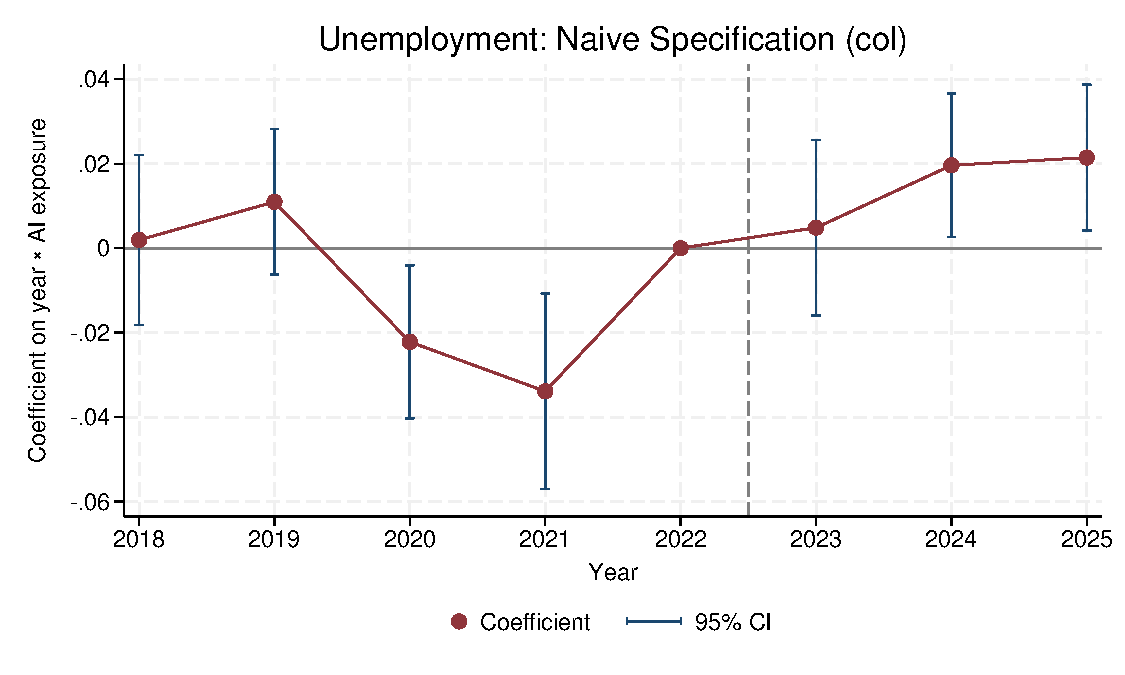
\includegraphics[width=0.88\textwidth]{unemp_naive_plot_col.pdf}
\caption{Unemployment: DiD coefficients (year $\times$ AI exposure), naive specification --- college subsample. Year 2022 is the baseline ($\hat\beta_{2022}\equiv 0$). Error bars are 95\% confidence intervals, standard errors clustered at the occupation level.}
\label{fig:unemp_naive_col}
\end{center}
\smallskip
\noindent\footnotesize\textit{Notes:} College subsample (BA or above). No additional controls.
\end{figure}

\begin{figure}[H]
\begin{center}
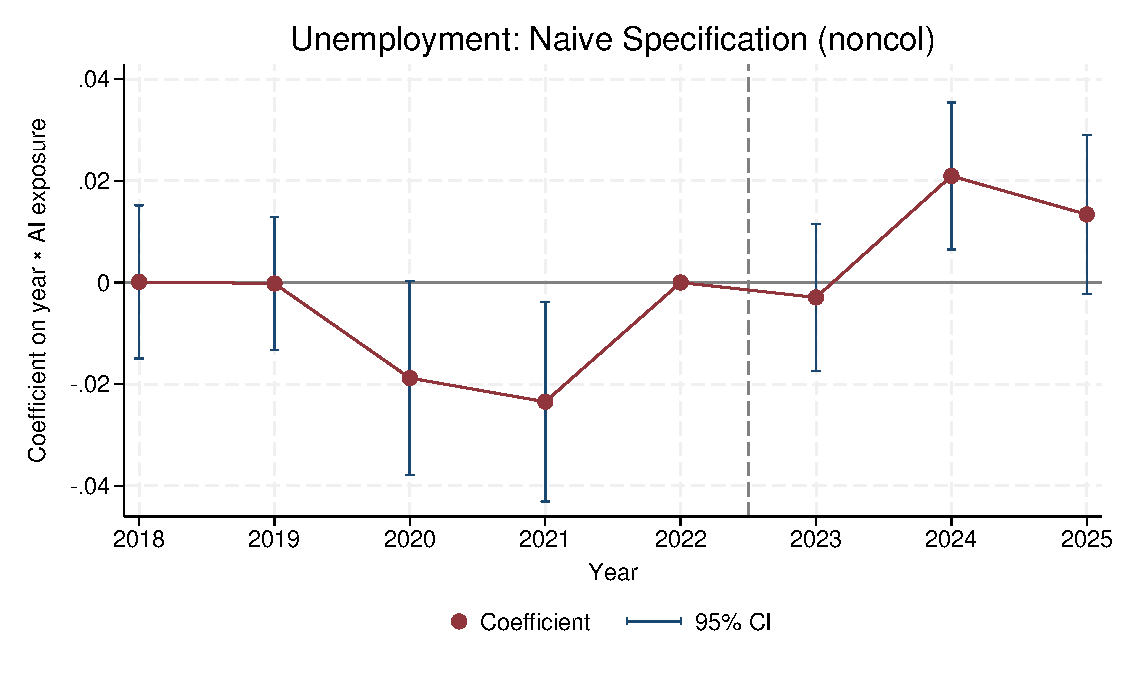
\includegraphics[width=0.88\textwidth]{unemp_naive_plot_noncol.pdf}
\caption{Unemployment: DiD coefficients (year $\times$ AI exposure), naive specification --- non-college subsample. Year 2022 is the baseline. Error bars are 95\% confidence intervals, standard errors clustered at the occupation level.}
\label{fig:unemp_naive_noncol}
\end{center}
\smallskip
\noindent\footnotesize\textit{Notes:} Non-college subsample (high school or some college). No additional controls.
\end{figure}

\begin{figure}[H]
\begin{center}
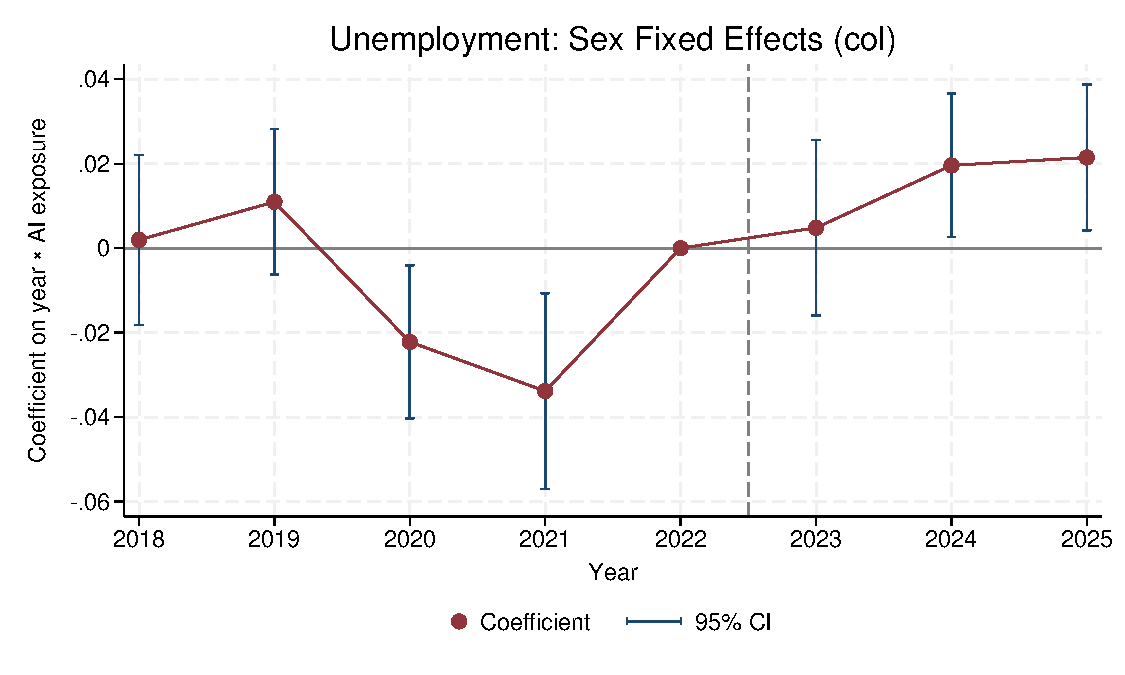
\includegraphics[width=0.88\textwidth]{unemp_sexFE_plot_col.pdf}
\caption{Unemployment: DiD coefficients (year $\times$ AI exposure), sex fixed effects --- college subsample. Year 2022 is the baseline. Error bars are 95\% confidence intervals, standard errors clustered at the occupation level.}
\label{fig:unemp_sexFE_col}
\end{center}
\smallskip
\noindent\footnotesize\textit{Notes:} College subsample. Sex fixed effects absorbed via \texttt{reghdfe}.
\end{figure}

\begin{figure}[H]
\begin{center}
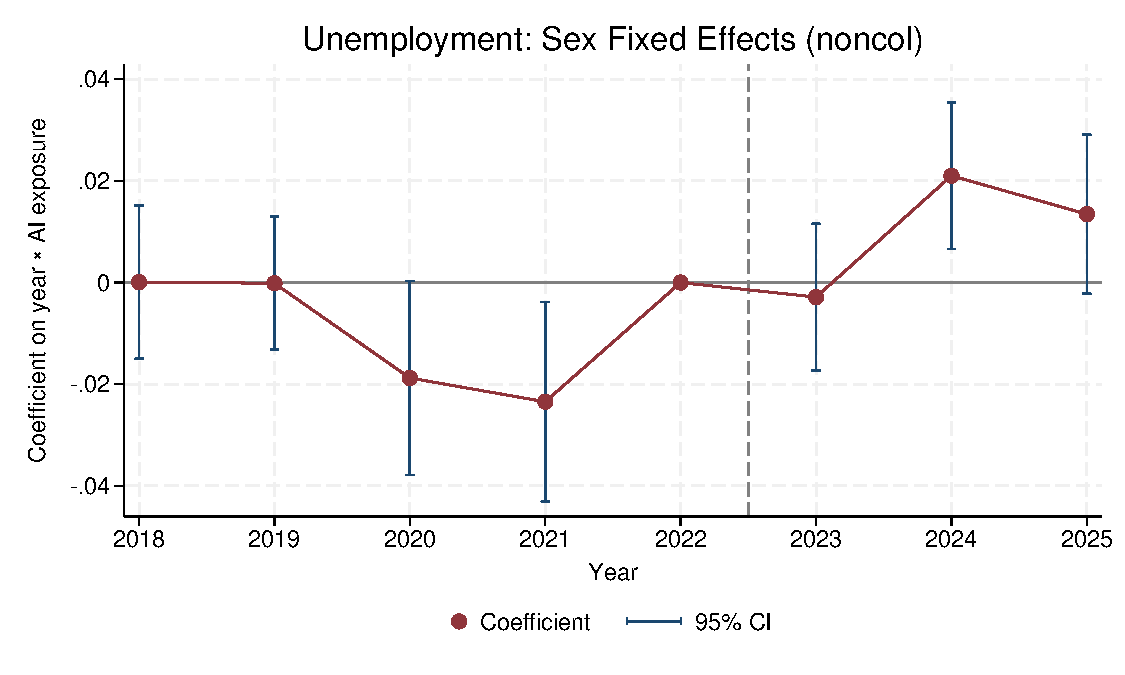
\includegraphics[width=0.88\textwidth]{unemp_sexFE_plot_noncol.pdf}
\caption{Unemployment: DiD coefficients (year $\times$ AI exposure), sex fixed effects --- non-college subsample. Year 2022 is the baseline. Error bars are 95\% confidence intervals, standard errors clustered at the occupation level.}
\label{fig:unemp_sexFE_noncol}
\end{center}
\smallskip
\noindent\footnotesize\textit{Notes:} Non-college subsample. Sex fixed effects absorbed via \texttt{reghdfe}.
\end{figure}

\begin{figure}[H]
\begin{center}
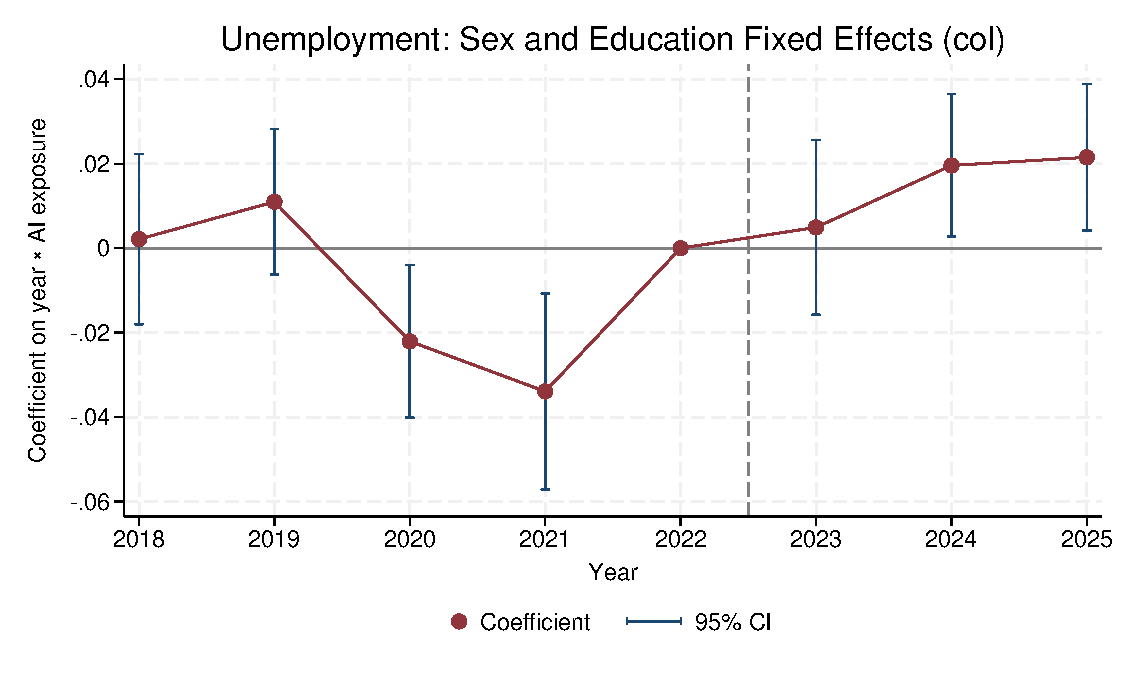
\includegraphics[width=0.88\textwidth]{unemp_sexeducFE_plot_col.pdf}
\caption{Unemployment: DiD coefficients (year $\times$ AI exposure), sex and education fixed effects --- college subsample. Year 2022 is the baseline. Error bars are 95\% confidence intervals, standard errors clustered at the occupation level.}
\label{fig:unemp_sexeducFE_col}
\end{center}
\smallskip
\noindent\footnotesize\textit{Notes:} College subsample. Sex and education fixed effects absorbed. Within the college subsample, education FE absorbs differences across BA, MA, Professional, and PhD.
\end{figure}

\begin{figure}[H]
\begin{center}
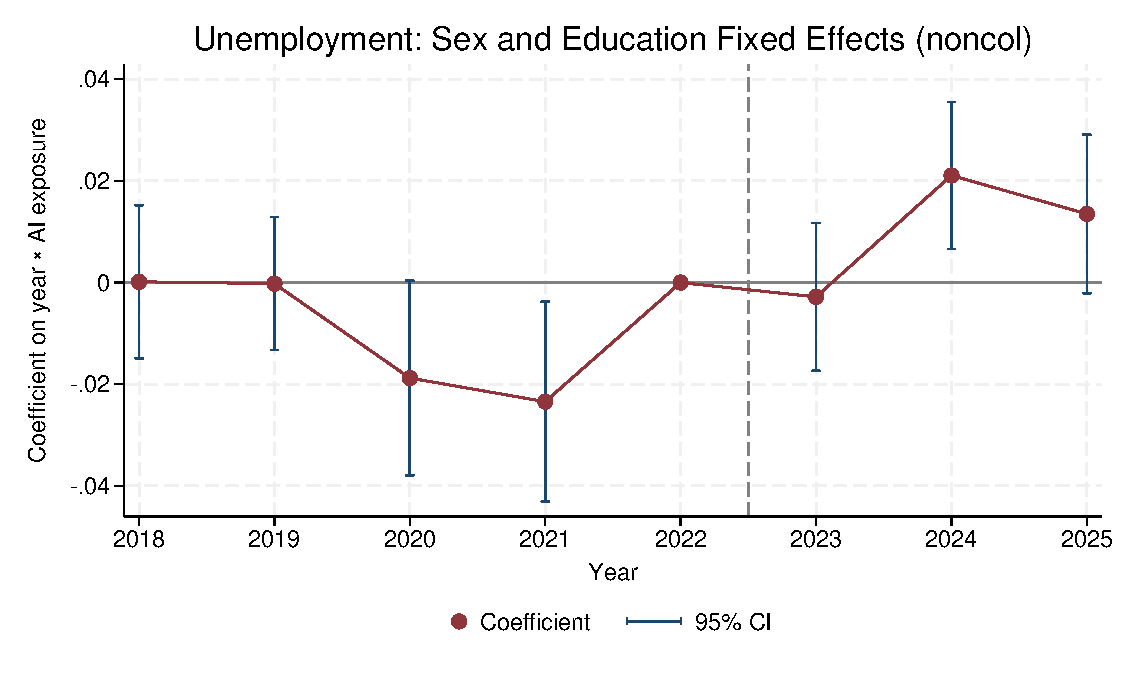
\includegraphics[width=0.88\textwidth]{unemp_sexeducFE_plot_noncol.pdf}
\caption{Unemployment: DiD coefficients (year $\times$ AI exposure), sex and education fixed effects --- non-college subsample. Year 2022 is the baseline. Error bars are 95\% confidence intervals, standard errors clustered at the occupation level.}
\label{fig:unemp_sexeducFE_noncol}
\end{center}
\smallskip
\noindent\footnotesize\textit{Notes:} Non-college subsample. Sex and education fixed effects absorbed. Within the non-college subsample, education FE absorbs differences across high school and some-college categories.
\end{figure}

\clearpage

%==================================================
\section{Log Wage Coefficient Plots --- Separate Subsamples}
%==================================================

\begin{figure}[H]
\begin{center}
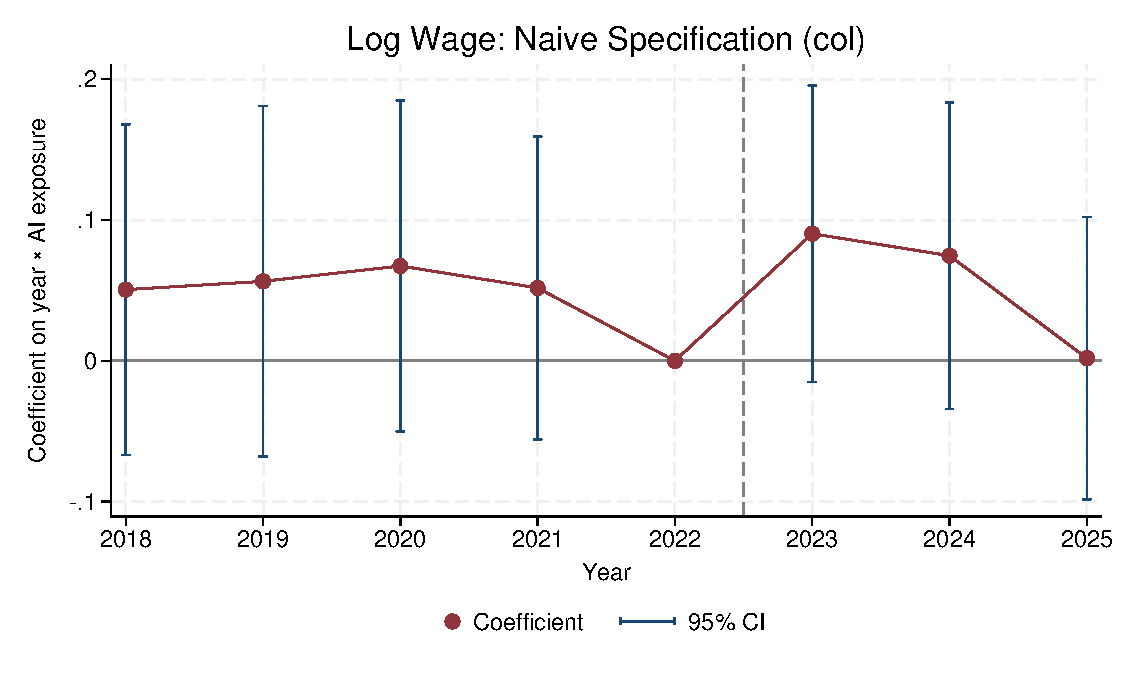
\includegraphics[width=0.88\textwidth]{lw_naive_plot_col.pdf}
\caption{Log Wage: DiD coefficients (year $\times$ AI exposure), naive specification --- college subsample. Year 2022 is the baseline ($\hat\beta_{2022}\equiv 0$). Error bars are 95\% confidence intervals, standard errors clustered at the occupation level.}
\label{fig:lw_naive_col}
\end{center}
\smallskip
\noindent\footnotesize\textit{Notes:} College subsample (BA or above). No additional controls. Observations with zero or missing wage income excluded.
\end{figure}

\begin{figure}[H]
\begin{center}
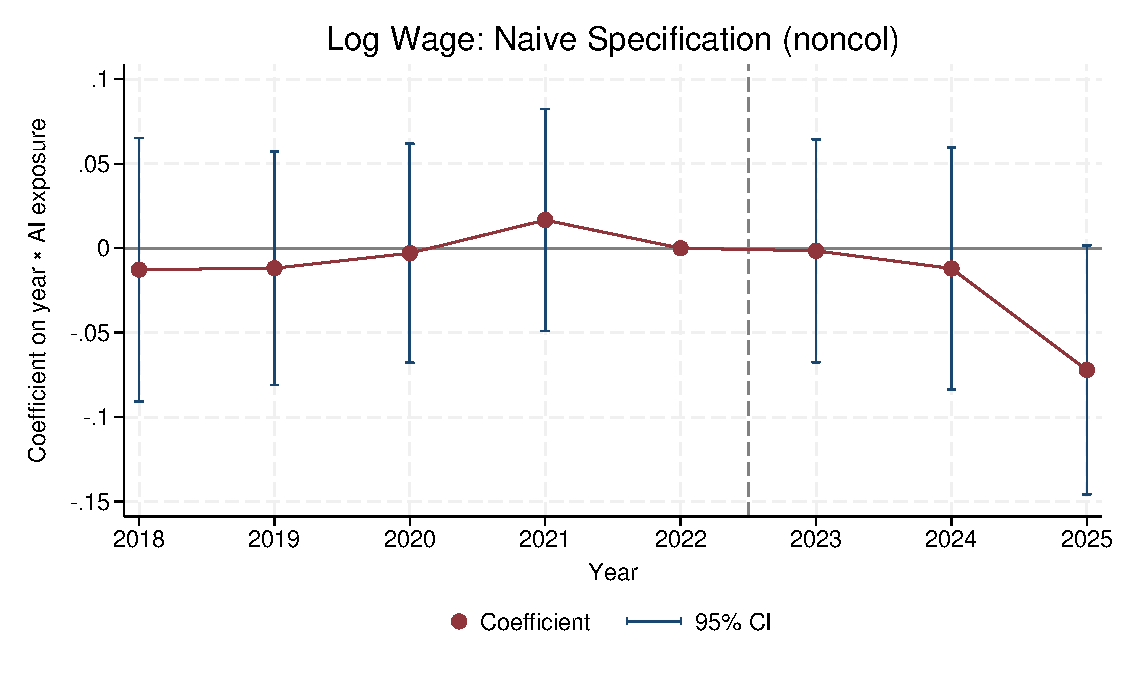
\includegraphics[width=0.88\textwidth]{lw_naive_plot_noncol.pdf}
\caption{Log Wage: DiD coefficients (year $\times$ AI exposure), naive specification --- non-college subsample. Year 2022 is the baseline. Error bars are 95\% confidence intervals, standard errors clustered at the occupation level.}
\label{fig:lw_naive_noncol}
\end{center}
\smallskip
\noindent\footnotesize\textit{Notes:} Non-college subsample. No additional controls. Observations with zero or missing wage income excluded.
\end{figure}

\begin{figure}[H]
\begin{center}
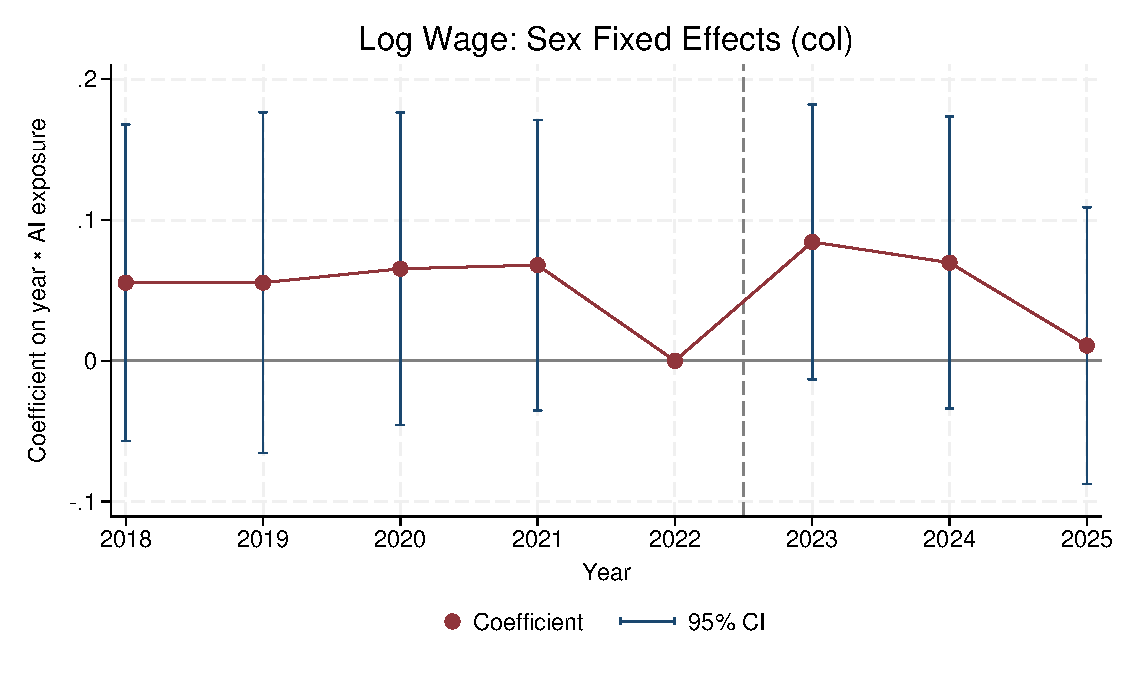
\includegraphics[width=0.88\textwidth]{lw_sexFE_plot_col.pdf}
\caption{Log Wage: DiD coefficients (year $\times$ AI exposure), sex fixed effects --- college subsample. Year 2022 is the baseline. Error bars are 95\% confidence intervals, standard errors clustered at the occupation level.}
\label{fig:lw_sexFE_col}
\end{center}
\smallskip
\noindent\footnotesize\textit{Notes:} College subsample. Sex fixed effects absorbed via \texttt{reghdfe}.
\end{figure}

\begin{figure}[H]
\begin{center}
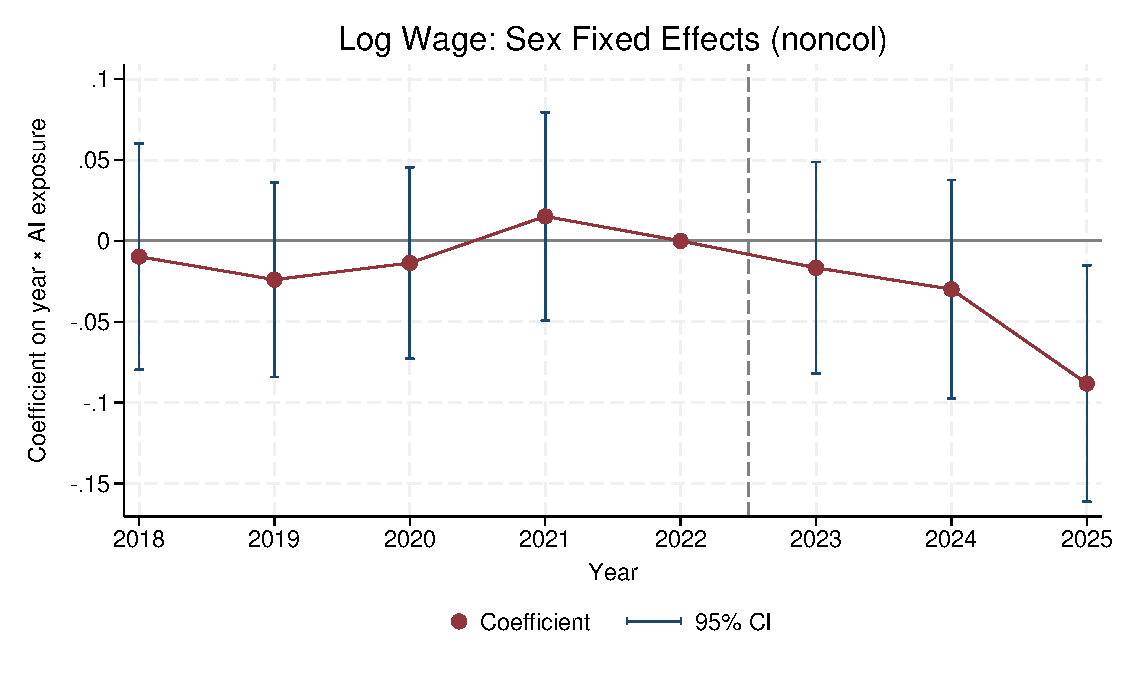
\includegraphics[width=0.88\textwidth]{lw_sexFE_plot_noncol.pdf}
\caption{Log Wage: DiD coefficients (year $\times$ AI exposure), sex fixed effects --- non-college subsample. Year 2022 is the baseline. Error bars are 95\% confidence intervals, standard errors clustered at the occupation level.}
\label{fig:lw_sexFE_noncol}
\end{center}
\smallskip
\noindent\footnotesize\textit{Notes:} Non-college subsample. Sex fixed effects absorbed via \texttt{reghdfe}.
\end{figure}

\begin{figure}[H]
\begin{center}
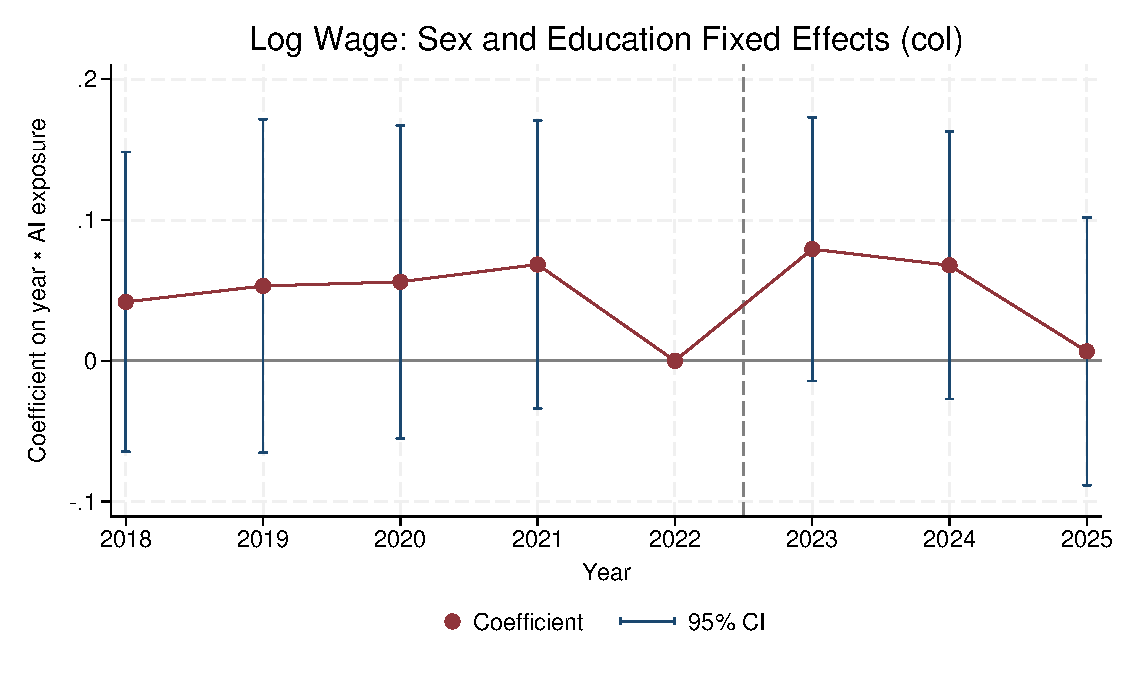
\includegraphics[width=0.88\textwidth]{lw_sexeducFE_plot_col.pdf}
\caption{Log Wage: DiD coefficients (year $\times$ AI exposure), sex and education fixed effects --- college subsample. Year 2022 is the baseline. Error bars are 95\% confidence intervals, standard errors clustered at the occupation level.}
\label{fig:lw_sexeducFE_col}
\end{center}
\smallskip
\noindent\footnotesize\textit{Notes:} College subsample. Sex and education fixed effects absorbed.
\end{figure}

\begin{figure}[H]
\begin{center}
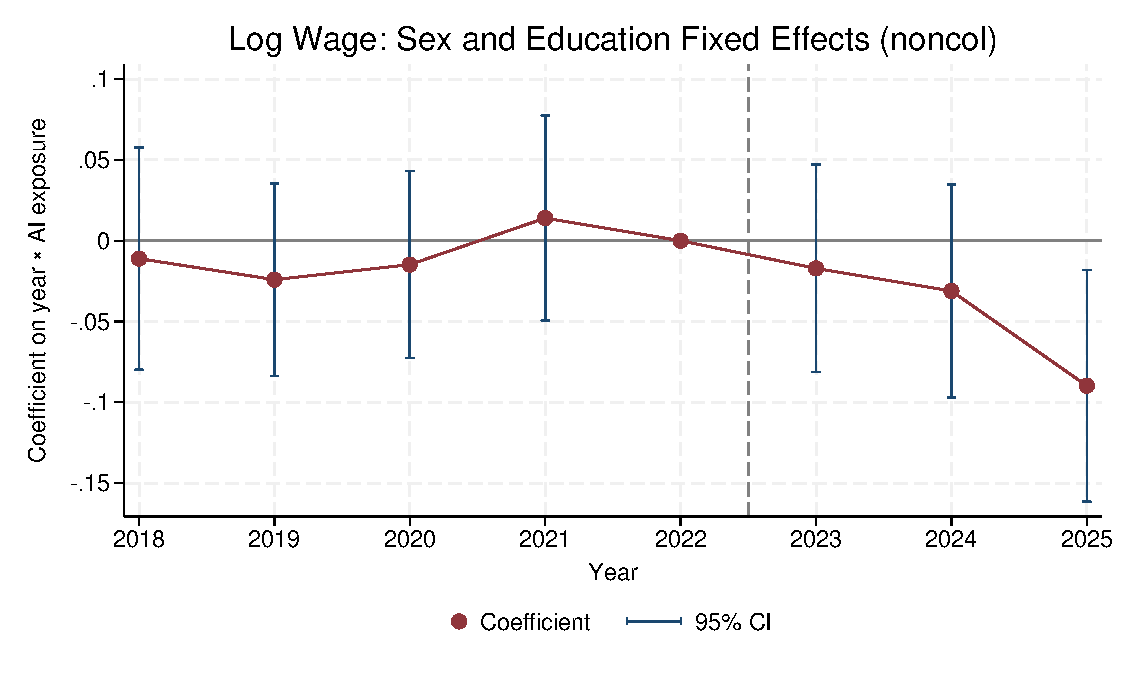
\includegraphics[width=0.88\textwidth]{lw_sexeducFE_plot_noncol.pdf}
\caption{Log Wage: DiD coefficients (year $\times$ AI exposure), sex and education fixed effects --- non-college subsample. Year 2022 is the baseline. Error bars are 95\% confidence intervals, standard errors clustered at the occupation level.}
\label{fig:lw_sexeducFE_noncol}
\end{center}
\smallskip
\noindent\footnotesize\textit{Notes:} Non-college subsample. Sex and education fixed effects absorbed.
\end{figure}

\clearpage

%==================================================
\section{Change in Unemployment, 2023--2025}
%==================================================

\begin{figure}[H]
\begin{center}
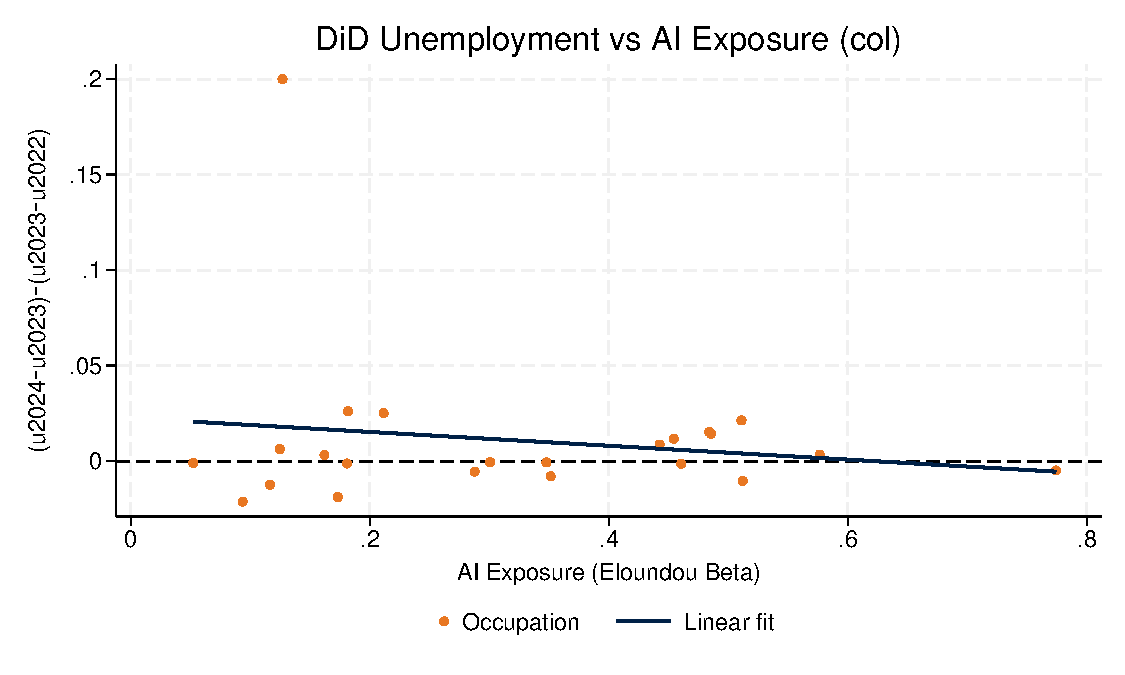
\includegraphics[width=0.88\textwidth]{delta_unemp_did_col.pdf}
\caption{DiD unemployment vs.\ AI exposure, college subsample. Vertical axis: $(u_{2024}-u_{2023})-(u_{2023}-u_{2022})$ by major occupation group. Each point is one occupation group; line is an OLS fit.}
\label{fig:delta_col}
\end{center}
\smallskip
\noindent\footnotesize\textit{Notes:} College subsample (educ $>$ 110). Occupation-group unemployment rates are simple means within the subsample. The DiD measure nets out the pre-period trend $(u_{2023}-u_{2022})$ from the post-period change $(u_{2024}-u_{2023})$, isolating the acceleration in unemployment relative to the pre-AI baseline. AI exposure is the group-mean Eloundou et al.\ (2024) GPT-4 beta score.
\end{figure}

\begin{figure}[H]
\begin{center}
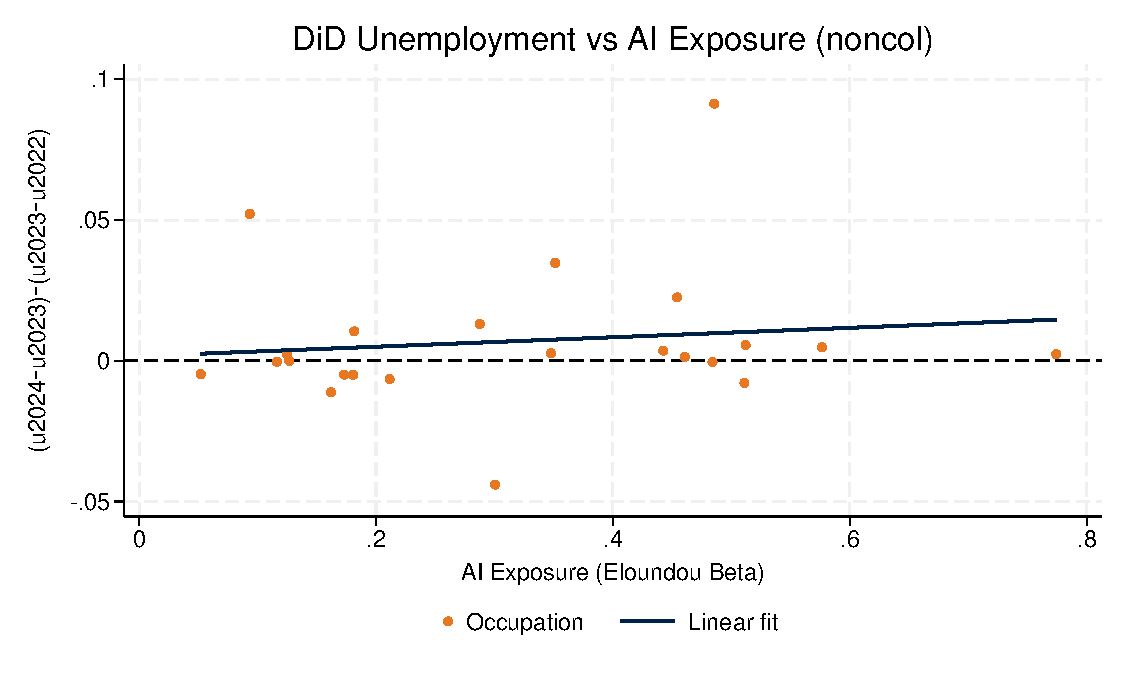
\includegraphics[width=0.88\textwidth]{delta_unemp_did_noncol.pdf}
\caption{DiD unemployment vs.\ AI exposure, non-college subsample. Vertical axis: $(u_{2024}-u_{2023})-(u_{2023}-u_{2022})$ by major occupation group. Each point is one occupation group; line is an OLS fit.}
\label{fig:delta_noncol}
\end{center}
\smallskip
\noindent\footnotesize\textit{Notes:} Non-college subsample (educ $\leq$ 110). Occupation-group unemployment rates are simple means within the subsample. The DiD measure nets out the pre-period trend from the post-period change. AI exposure is the group-mean Eloundou et al.\ (2024) GPT-4 beta score.
\end{figure}

\end{document}
